\section*{Experiment 2: Deductive Reasoning (Wason Selection Task)}

\subsection*{2.1. Experimental Setup and Protocol}
\textbf{Objective:} To evaluate the ability to apply \textit{Modus Tollens} in abstract vs. social contexts and identify systematic cognitive biases in LLM reasoning.

\textbf{Task Structure:}
The model is presented with a conditional rule: "If $P$, then $Q$." It is then shown four cards representing the cases $P$, $\neg P$, $Q$, and $\neg Q$. 
\textbf{Target:} Identify the \textit{minimum} number of cards that must be flipped to verify whether the rule is violated.
\textbf{Correct Answer:} $P$ and $\neg Q$ (the only cases that can falsify the rule).

\textbf{Content Manipulation (5 Conditions):}
To control for data contamination and test the "Deontic Selection" hypothesis, we used five stimulus datasets (100 rules each):
\begin{itemize}
    \item \textbf{FL Canonical:} Standard abstract symbols (letters/numbers) common in literature.
    \item \textbf{FL Neutral:} Decontaminated abstract pairs (e.g., "If the symbol is an Arrow, then the pattern is Striped").
    \item \textbf{Concrete Facts:} Verifiable real-world properties (e.g., "If an animal is a dolphin, it breathes air").
    \item \textbf{Familiar Social:} Well-known social norms (e.g., "If a person is driving, they must have a license").
    \item \textbf{Unfamiliar Fantasy Social:} Deontic rules set in fictional worlds (e.g., "If a traveler crosses the Moon Gate, they must carry a Silver Feather"). This tests if models recognize the \textit{structure} of a social contract without prior knowledge.
\end{itemize}

\textbf{Prompt Conditions:}
\begin{itemize}
    \item \textbf{Neutral:} Format-only instruction. Serves as the baseline for "raw" logic.
    \item \textbf{Assisted Falsification:} Priming the model as a "logic expert" with a directive to find violations.
    \item \textbf{Chain-of-Thought (CoT):} Step-by-step reasoning before the final answer.
\end{itemize}

\subsection*{2.2. Quantitative Results: Performance and Consistency}
We utilized 500 trials per model per condition (100 rules $\times$ 5 permutations of card order). This allowed us to measure the \textbf{Consistency Rate} --- the percentage of rules where the model gives identical answers regardless of card order.

\begin{table}[h!]
\centering
\caption{Wason Selection Task Performance (EMA) across all content conditions}
\label{tab:wason_full_data}
\begin{tabular}{lccccc}
\toprule
\textbf{Model} & \textbf{FL Neutral} & \textbf{FL Canon} & \textbf{Conc. Facts} & \textbf{Fam. Social} & \textbf{Unf. Fantasy} \\ 
\midrule
gpt-5.2           & 0.972 & 0.973 & 0.976 & 0.996 & 0.978 \\
qwen3-next-80b    & 0.976 & 0.933 & 0.980 & 0.946 & 0.938 \\
qwen3.5-397b      & 0.818 & 0.867 & 0.909 & 0.982 & 0.986 \\
claude-sonnet-4.6 & 0.898 & 0.907 & 0.956 & 0.982 & 0.970 \\
deepseek-v3.2     & 0.880 & 0.847 & 0.883 & 0.922 & 0.882 \\
grok-4.1-fast     & 0.720 & 0.647 & 0.875 & 0.818 & 0.818 \\
gemma-3-27b-it    & 0.578 & 0.553 & 0.792 & 0.904 & 0.888 \\
glm-4.7-flash     & 0.614 & 0.533 & 0.562 & 0.686 & 0.590 \\
gemma-3-12b-it    & 0.106 & 0.207 & 0.380 & 0.546 & 0.436 \\
\bottomrule
\end{tabular}
\end{table}

\subsection*{2.3. Analysis of Cognitive Biases: MBI and CBR}
We distinguished between \textbf{Matching Bias Index (MBI)} (choosing cards mentioned in the rule, $P$ and $Q$) and \textbf{Confirmation Bias Rate (CBR)} (choosing only $P$).

\begin{table}[h!]
\centering
\caption{Matching Bias (MBI) and Confirmation Bias (CBR) in FL Neutral}
\label{tab:wason_bias}
\begin{tabular}{lcccc}
\toprule
\textbf{Model} & \textbf{EMA} & \textbf{MBI} & \textbf{CBR} & \textbf{Bias Index (MBI+CBR)} \\ 
\midrule
gemma-3-12b-it    & 0.106 & 0.516 & 0.020 & 0.536 \\
gemma-3-27b-it    & 0.578 & 0.296 & 0.000 & 0.296 \\
glm-4.7-flash     & 0.614 & 0.190 & 0.040 & 0.230 \\
claude-sonnet-4.6 & 0.898 & 0.078 & 0.000 & 0.078 \\
gpt-5.2           & 0.972 & 0.000 & 0.004 & 0.004 \\
\bottomrule
\end{tabular}
\end{table}

\subsection*{2.4. Qualitative Error Classification}
To understand failure modes, we categorized answers into six types. Below are typical examples from the weaker models in the FL Neutral condition:

\begin{enumerate}
    \item \textbf{CORRECT:} $\{P, \neg Q\}$. (e.g., Qwen-80b: \texttt{['A', '7']}).
    \item \textbf{MATCHING BIAS:} $\{P, Q\}$ --- Choosing cards explicitly named. (e.g., gemma-12b: \texttt{['A', '4']} for the rule "If vowel, then even").
    \item \textbf{CONFIRMATION BIAS:} $\{P\}$ --- Minimal confirmation. (e.g., glm-4.7: \texttt{['A']}).
    \item \textbf{LOGIC ERROR:} e.g., $\{\neg P, \neg Q\}$ or $\{\neg P, Q\}$. (e.g., gemma-12b: \texttt{['B', '7']} --- total inversion).
    \item \textbf{OVER-SELECTION:} e.g., $\{P, Q, \neg Q\}$. Attempting to "be safe" by flipping too many cards.
    \item \textbf{ALL CARDS:} Extreme uncertainty.
\end{enumerate}

\subsection*{2.5. The Impact of Prompting and CoT}
For the majority of models, CoT significantly improved EMA (e.g., \texttt{claude-sonnet-4.6} $+0.180$, \texttt{deepseek-v3.2} $+0.278$). However, for weaker open models, the effect was \textit{negative}:

\begin{table}[h!]
\centering
\caption{Comparison of Neutral vs. CoT Prompts in FL Neutral}
\label{tab:wason_prompts}
\begin{tabular}{lccc}
\toprule
\textbf{Model} & \textbf{EMA (Neutral)} & \textbf{EMA (CoT)} & \textbf{$\Delta$EMA} \\ 
\midrule
gpt-5.2            & 0.884 & 0.976 & +0.092 \\
claude-sonnet-4.6  & 0.790 & 0.970 & +0.180 \\
deepseek-v3.2      & 0.658 & 0.936 & +0.278 \\
glm-4.7-flash      & 0.332 & 0.258 & -0.074 \\
gemma-3-27b-it     & 0.406 & 0.368 & -0.038 \\
\bottomrule
\end{tabular}
\end{table}

\subsection*{2.6. Key Findings: Deontic Facilitation}
The results strongly support the \textbf{Pragmatic Schemas} hypothesis. The median accuracy gain when moving from abstract to "Unfamiliar Fantasy Social" rules was $+0.072$. This proves that LLMs identify the \textit{deontic structure} (obligation/permission) rather than just recalling training data.

\subsection*{2.7. Visualization of Effects}

\begin{figure}[h!]
\centering
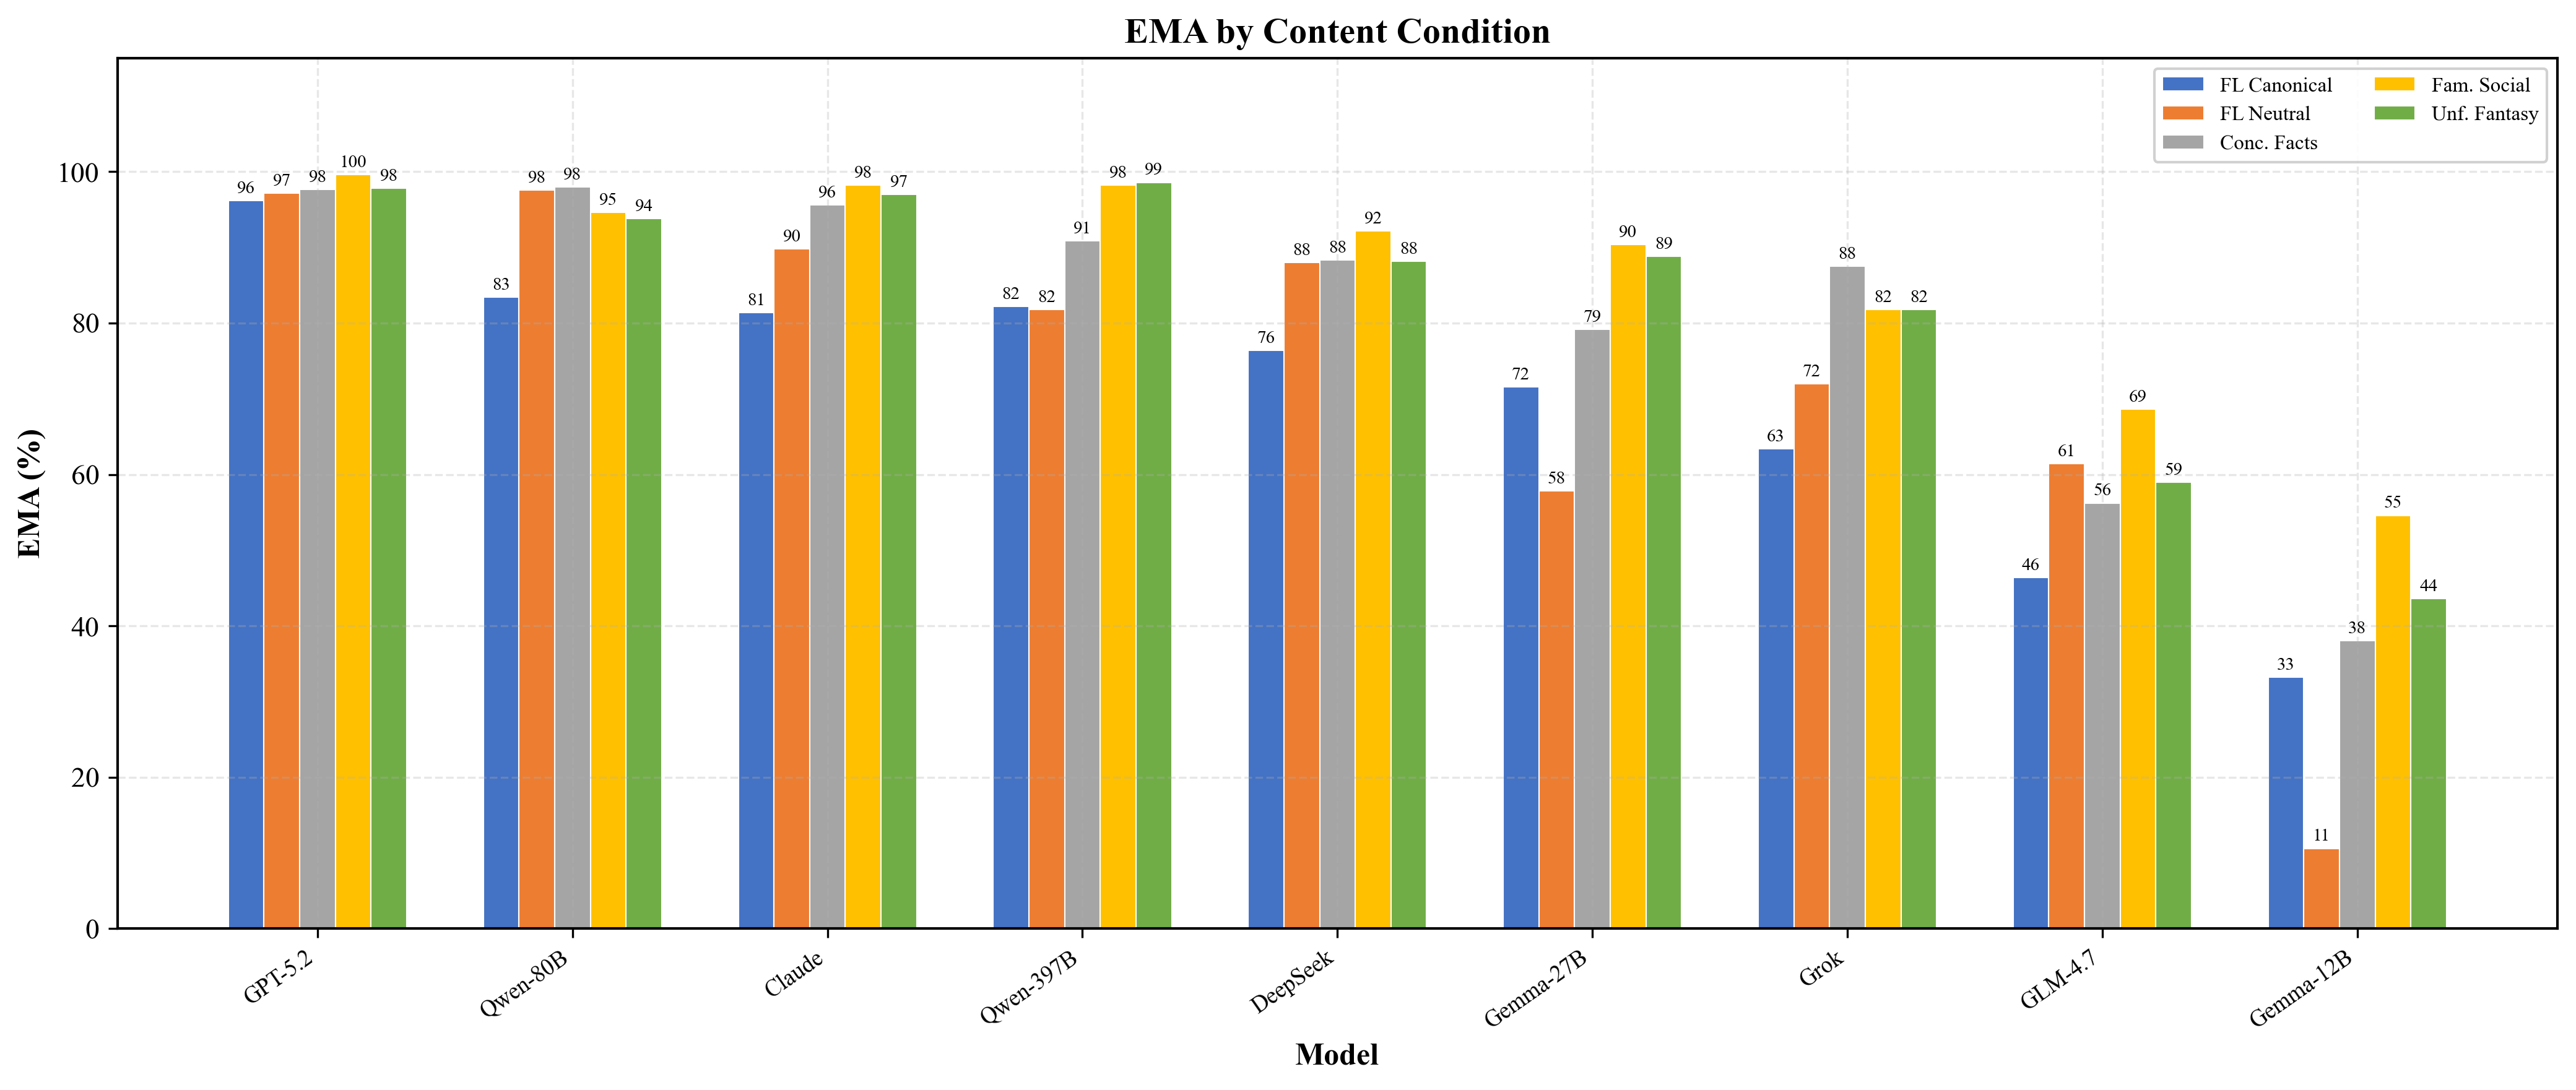
\includegraphics[width=0.6\textwidth]{../experiments_raw_results/wason-selection/figures/wason_ema_conditions.png}
\caption{The "Content Effect": Accuracy significantly increases when moving from abstract logic to social norms.}
\end{figure}

\begin{figure}[h!]
\centering
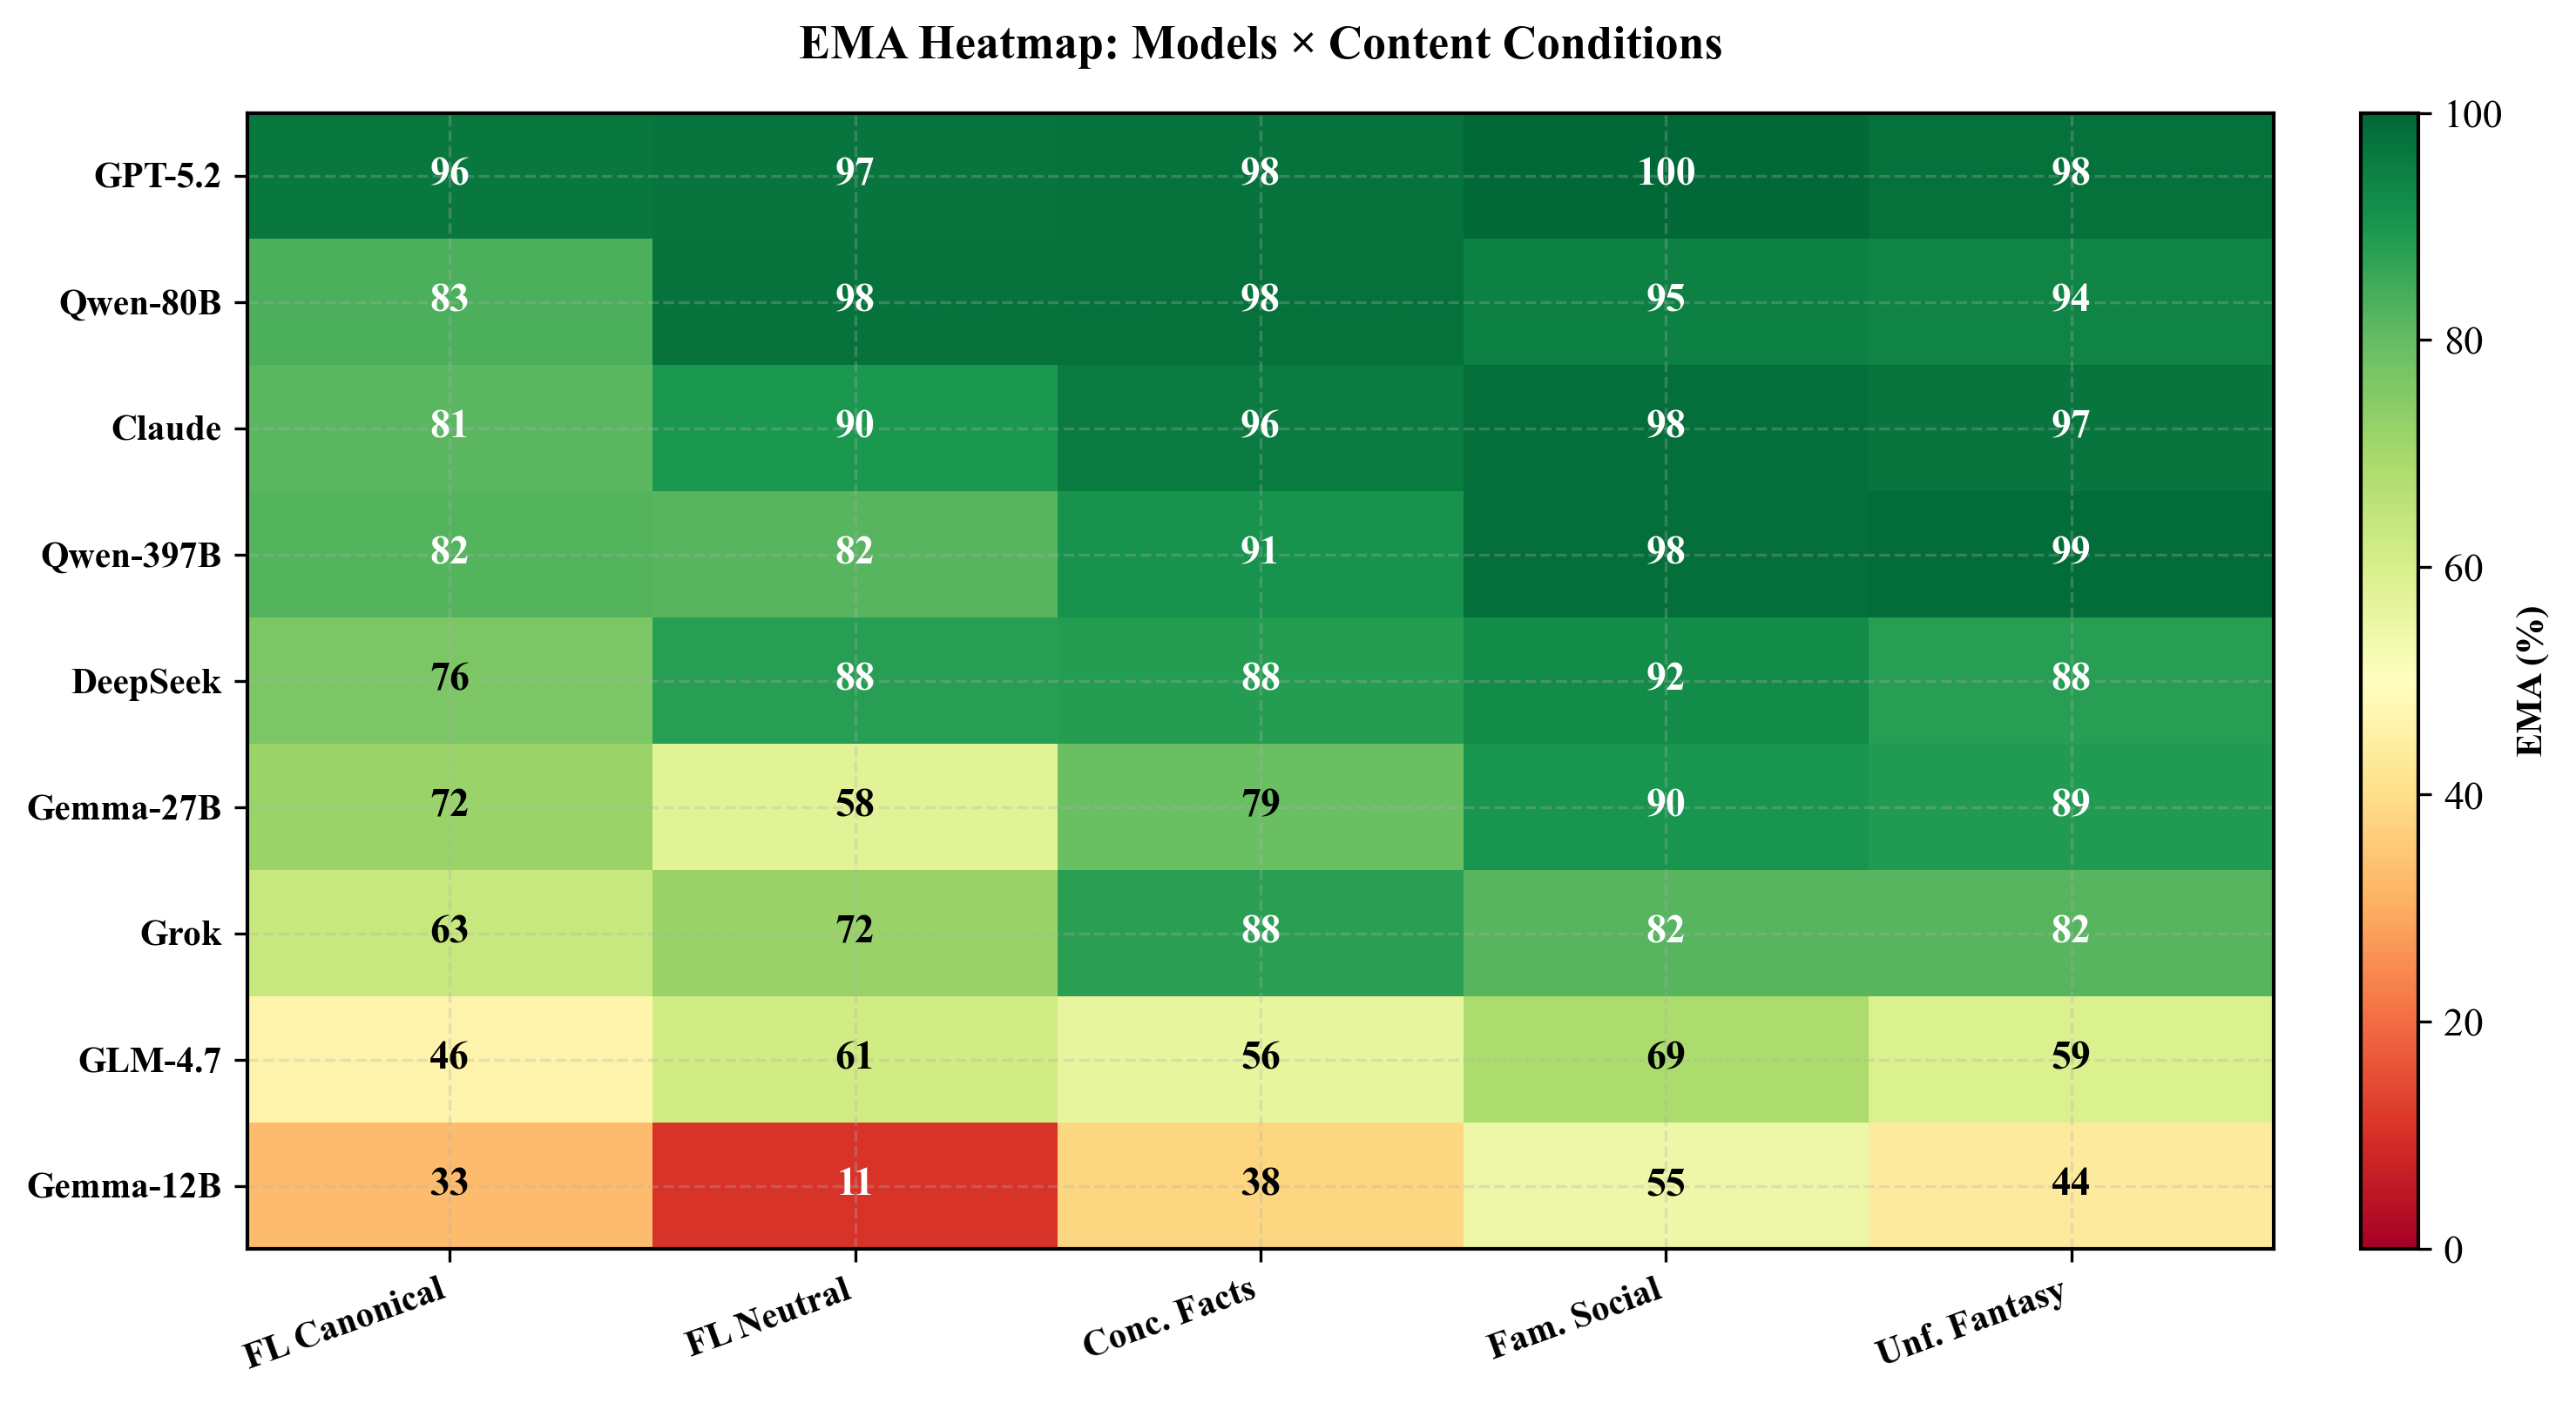
\includegraphics[width=0.48\textwidth]{../experiments_raw_results/wason-selection/figures/wason_ema_heatmap.png}
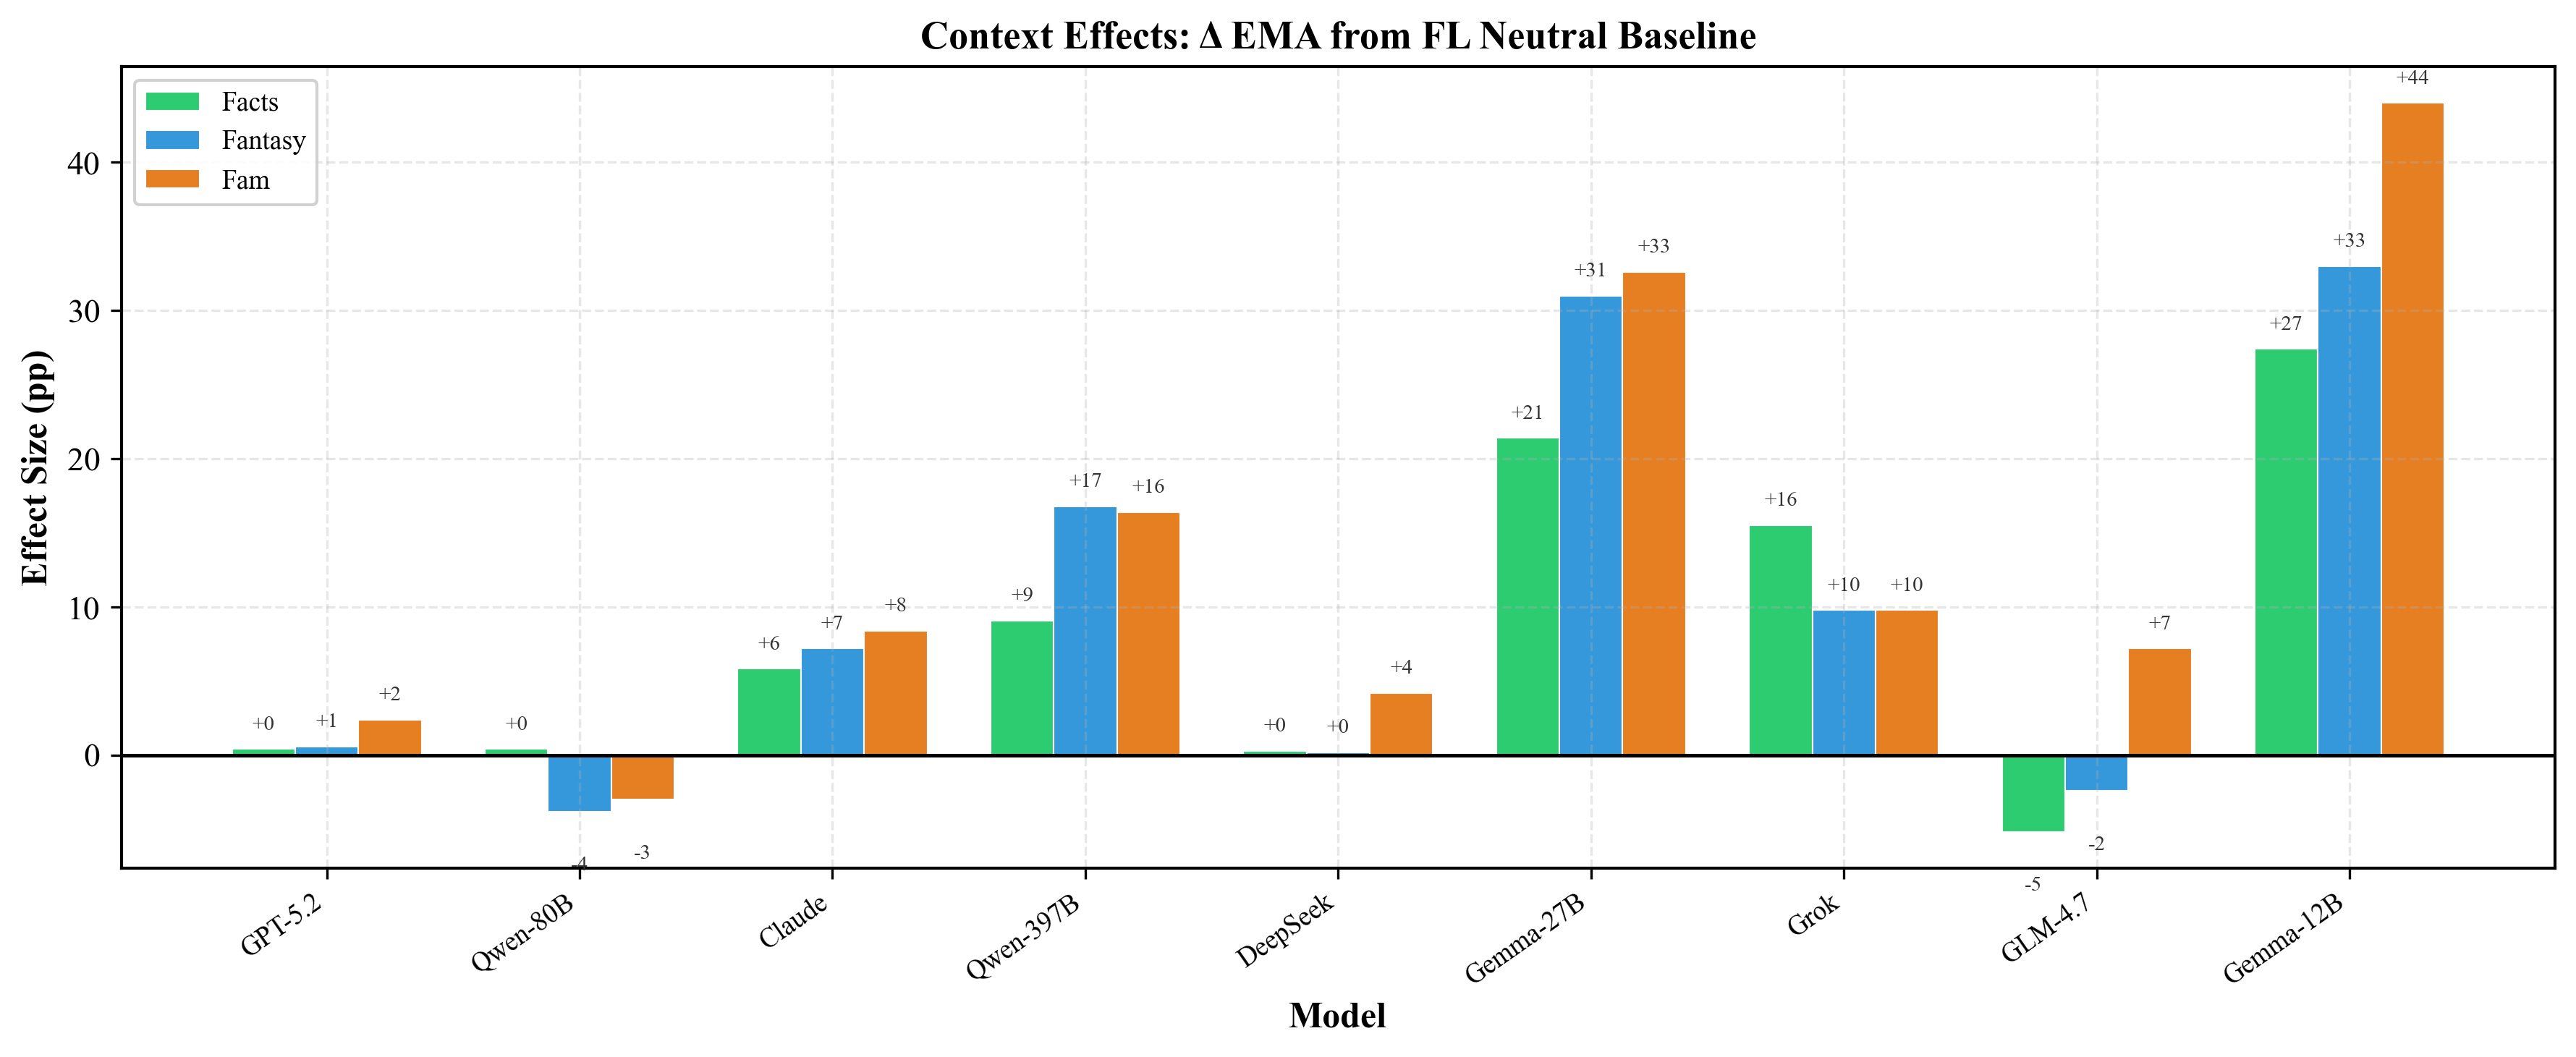
\includegraphics[width=0.48\textwidth]{../experiments_raw_results/wason-selection/figures/wason_context_effects.png}
\caption{Left: Heatmap of accuracy. Right: Delta gain from social content.}
\end{figure}
...
